\section{Experimental results}\label{sec:experiments}

In this section, we provide an experimental evaluation of our algorithms based on two classes of test instances. More precisely, we test our approach on two IRMDPs: (1) Random MDPs (\texttt{Random})  and (2) Diamond MDPs (\texttt{Diamond}).
%\item Grid MDPs (\texttt{Grid}).

For a given MDP, let $MR(f^{\hat{\pi}}, \mathcal{R})$ be the maximum regret of the rounding deterministic policy and $MR(f^{\pi^*}, \mathcal{R})$  be the maximum regret of the optimal deterministic policy. We define the Value Ratio of such MDPs as: $VR = \dfrac{MR(f^{\hat{\pi}}, \mathcal{R})}{MR(f^{\pi^*}, \mathcal{R})}\;$.
Moreover, let $\hat{T}$ (respectively $T^*$) be the computing time necessary to calculate the rounding (respectively optimal) deterministic policy, we define the Time Ratio as: $TR=\dfrac{T^*}{\hat{T}}\;$.
\begin{table}[h] % <-- HERE
 \setlength{\tabcolsep}{2.5pt}
 \renewcommand \arraystretch{1.1}
\begin{center}
\begin{tabular}{rrrrrrrrrrrrrrrrrrrrrrrrrrrr}
	&		&				&				&				&	\multicolumn{2}{c}{	\texttt{Comp. Time}}	\\
$|S|$	&	$|A|$	&		\texttt{VR}		&		\texttt{TR}		&		\texttt{\% diff}		&	\texttt{Base}	&	\texttt{C\&B}	\\
\cmidrule(lr){1-2} \cmidrule(lr){3-3} \cmidrule(lr){4-4}  \cmidrule(lr){5-5}  \cmidrule(lr){6-7}
5	&	2	&			1.07	&			1.83	&			50\%	&	2.59	&	2.27	\\
	&	3	&			1.03	&			2.44	&			20\%	&	5.05	&	5.11	\\
	&	4	&			1.09	&			2.17	&			50\%	&	5.28	&	4.67	\\
	&	5	&			1.07	&			2.85	&			50\%	&	8.03	&	7.99	\\
	&	10	&			1.02	&			2.50	&			30\%	&	13.76	&	12.61	\\
\cmidrule(lr){1-2} \cmidrule(lr){3-3} \cmidrule(lr){4-4}  \cmidrule(lr){5-5}  \cmidrule(lr){6-7}
10	&	2	&			1.11	&			4.11	&			90\%	&	21.78	&	20.12	\\
	&	3	&			1.15	&			7.63	&			80\%	&	81.67	&	73.43	\\
	&	4	&			1.04	&			9.19	&			60\%	&	312.05	&	266.35	\\
	&	5	&			1.06	&			8.42	&			90\%	&	570.15	&	478.07	\\
	&	10	&			1.01	&			18.79	&			90\%	&	1886.05	&	986.71	\\
\cmidrule(lr){1-2} \cmidrule(lr){3-3} \cmidrule(lr){4-4}  \cmidrule(lr){5-5}  \cmidrule(lr){6-7}
15	&	2	&			1.04	&			6.91	&			60\%	&	94.95	&	82.59	\\
	&	3	&			1.05	&			18.75	&			80\%	&	2240.40	&	2024.85	\\
	&	4	&			1.01	&			20.04	&			80\%	&	5366.92	&	3181.01	\\
	&	5	&			1.03	&			32.10	&			100\%	&	7677.25	&	4127.52	\\
\cmidrule(lr){1-2} \cmidrule(lr){3-3} \cmidrule(lr){4-4}  \cmidrule(lr){5-5}  \cmidrule(lr){6-7}
	&	Avg.	&			1.06	&			7.77	&			70\%	&	1306.14	&	805.24	
\end{tabular}						
\end{center}
\caption{Time Ratio and Value Ratio for \texttt{Random} MDPs.}														\label{tab:random}								
\end{table} % <-- HERE
  
\subsection{Random MDPs}
\paragraph{Description}
A random MDP is defined by several parameters including its number of states $|S|$, its number of actions $|A|$. The rewards are bounded between randomly two real values. Transition function has several properties: from any state $s$ restrict transitions to reach $\lceil \log_2(n) \rceil$ states. For each pair of $(s, a)$ draw reachable states based on uniform distribution over the set of states. For drawn states, transition probabilities are formed based on Gaussian distribution. The initial state distribution $\beta$ is uniform and we choose discount factor $\gamma = 0.95$. 
\paragraph{Analysis of the results}
In Table~\ref{tab:random} we present the results concerning the performances of our algorithm on random MDP with $|S| \in \{5,10,15\}$ and $|A| \in \{2, 3, 4, 5, 10\}$. For each combination of states and actions, we provide the average results over $10$ different simulations. The first two columns report the Value Ratio and the Time Ratio (\texttt{VR} and \texttt{TR}). The column \texttt{\% diff} shows the percentage of cases where the optimal policy is different from the rounding policy. The final two columns show the computing time of the baseline branch-and-bound algorithm (\texttt{Base}) and the improved version (\texttt{C\&B}), presented in Section~\ref{sec:bb}.

We notice that in average, $70\%$ of the times the optimal deterministic policy differs from the rounding deterministic policy, while the maximum regret of the rounding deterministic policy is $6\%$ worse than the optimal deterministic policy. This moderate gap is probably due to the fact that random MDPs do not present a special structure. For such instances it is more unlikely to have extreme configurations like the one showed in Section~\ref{sec:comparison}.
Calculating the optimal deterministic policy is one order of magnitude slower than computing the rounding deterministic policy. On the other hand, the cut-and-branch version of the algorithm is almost two times faster than the basic version.  
%Finally, it is interesting to notice that in the basic implementation of the algorithm, the number of additional Benders cuts added during the branch-and-bound is significantly low (on average no more than $2$ cuts per node). This explains why the cut-and-branch version of the branch-and-bound algorithm performs better than the standard version.
 

\subsection{Diamond MDPs}
\paragraph{Description}
This class of MDPs has been introduced for the first time in Benavent and Zanuttini~\cite{benavent2018}. 
In this family of problems, the reward of a few states suffices to generate a lot of uncertainties about the optimal policy. This IRMDP is an interesting set of instances to test our proposed algorithm. 
This class of MDPs has a diamond structure, with one top and one bottom state (playing the role of start and terminal of the MDP), one intermediate layer of states, containing all the uncertainties on rewards, plus two intermediate layers between the extreme states and the intermediate layer. 

\begin{figure}[h]
\begin{center}
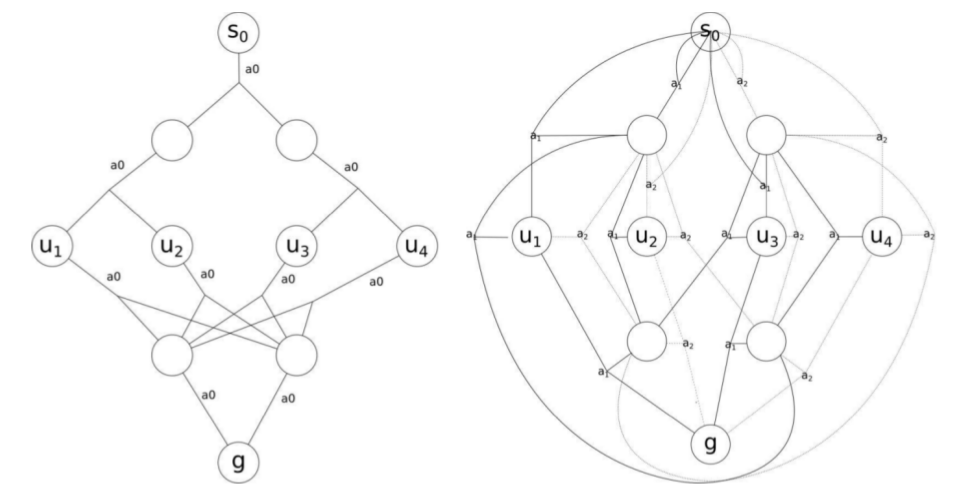
\includegraphics[width=8cm]{images/diamond.png}
\end{center}
\caption{Diamond MDP: actions $a_0$ (left) and $a_1, a_2$ (right) (Figure comes from \cite{benavent2018}).}
\label{fig:diamond}
\end{figure}

%\begin{wrapfigure}{r}{0.5\textwidth}
%\begin{center}
%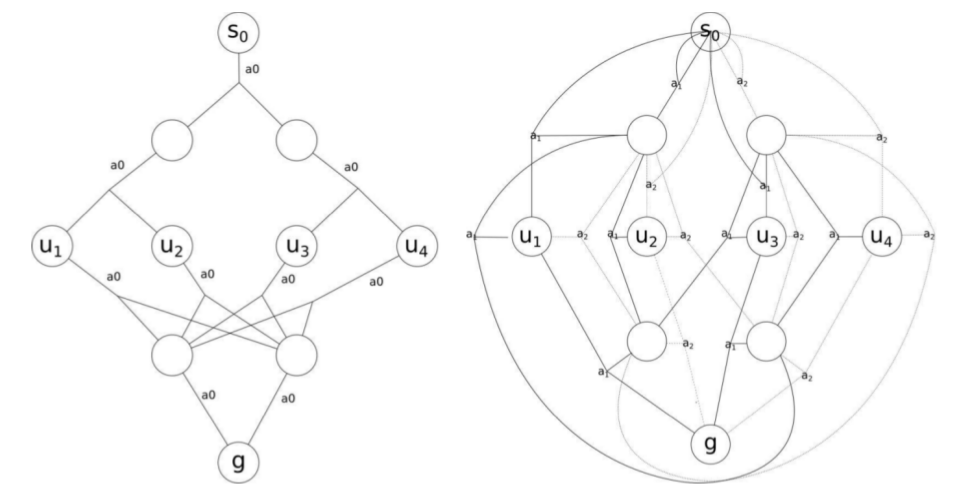
\includegraphics[width=8cm]{images/diamond.png}
%\end{center}
%\caption{Diamond MDP: actions $a_0$ (left) and $a_1, a_2$ (right). Figure comes from \cite{benavent2018}}
%\label{fig:diamond}
%\end{wrapfigure}


%From a point of viex of the parameters, the authors proposed to have that action $a_0$ would reach each child with a probability of $0.5$.
The diamond MDP structure is given in Figure~\ref{fig:diamond}. Action $a_0$ has probability $0.5$ to reach each child node.  
On the other hand $a_1$ (resp. $a_2$) has a probability of $p= 0.3$ (resp. $1-p$) to reach the left (resp. right) child node and to reach its parent otherwise.
The imprecise values of the rewards for the middle layer are $[-600,600]$, while the one of the bottom node is $[600,1000]$.

We propose a generalization of this family of MDP by testing a range of parameters for the probability $p \in \{0.05,0.10,\dots,0.40,0.45\}$. %We also introduce an additional intermediate layer, between the extreme states and the middle layer. In this way we have, in addition to $10$-states MDPs (callend one-level diamond MDPs) also  22-states MDPs (called two-level diamond MDPs). 

\paragraph{Analysis of the results}
In Table~\ref{tab:diamond}, we show how the Time Ratio and the Value ratio change with the increase of $p$.
It is clear that for Diamond MDPs the situation is different than for Random MDPs. In this case, the max regret of the rounding deterministic policy is $20\%$ worse than the one of the optimal deterministic policy. Moreover, the computing time for the optimal deterministic policy is less than one order of magnitude lower than the one needed by the rounding deterministic policy. These results show how, in presence of a specific structure, the difference between $MR(f^{\hat{\pi}}, \mathcal{R})$ and $MR(f^{\pi^*}, \mathcal{R})$ increases significantly.


\begin{table}[h]																	
 \centering
 \small
 \setlength{\tabcolsep}{4.0pt}
 \renewcommand \arraystretch{1.1}
\begin{tabular}{ccccccccccc}																					
\texttt{p}	&	5	&	10	&	15	&	20	&	25	&	30	&	35	&	40	&	45	&	Avg.	\\	
\cmidrule(lr){1-1} \cmidrule(lr){2-10} \cmidrule(lr){11-11}
\texttt{VR} &	1.66	&	1.24	&	1.16	&	1.13	&	1.15	&	1.15	&	1.15	&	1.14	&	1.16	&	\textbf{1.22}	\\	
\texttt{TR} &	10.23	&	7.44	&	6.32	&	6.48	&	7.67	&	5.93	&	7.62	&	10.46	&	13.80	&	\textbf{8.44}	\\	\\
\end{tabular}
\caption{Time Ratio and Value Ratio for \texttt{Diamond}.}														\label{tab:diamond}								
\end{table}																						



%\subsection{Grid MDPs}
%blablabla
%\paragraph{Description}
%blablabla
%\paragraph{Analysis of the results}
%blablabla



